\chapter{ Beschreibung d. Motorseglers, seiner Systeme und Anlagen}

\section{Einführung}
Der vorliegende Abschnitt enthält eine Beschreibung des Motorsegelflugzeuges und seiner Systeme, sowie der Standardausrüstung und Anlagen mit Benutzungshinweisen. 

\section{Steuerungsanlage im Cockpit}
Jeder Sitz ist ausgestattet mit Steuerknüppel, Seitenruderpedalen, Brems- und Wölbklappenhebel (jeweils links) und Ausklinkknopf (zwischen den Beinen).\\
Haubenverriegelung: Bedienhebel im Instrumentenpilz.\\
Haubennotabwurf: Zusätzlich zum Bedienhebel im Instrumentenpilz den roten Griff dahinter ziehen.\\
Die Bremse ist mit der Bremsklappe gekoppelt und wird im hinteren Bereich der Bremsklappen mit betätigt.\\
Die Trimmung ist in der Mittelkonsole angeordnet. Die Betätigung erfolgt durch Ziehen nach links und Verschieben des Hebels (Rastung durch Federkraft).\\
Die Lüftung befindet sich links und rechts neben den Sitzen. Die Betätigung erfolgt durch Entriegeln,  Ziehen nach hinten und Verriegeln\\

Zusätzlich verfügt die B13 über:

\begin{itemize}
\item Avionik Hauptschalter (Beschriftet mit EIN / AUS)
\item Propellerschlitten Hauptschalter / Noteinfahrschalter (Beschriftet mit Slide System)
\begin{itemize}
\item Vordere Position: Schlittensystem eingeschaltet (Das Schlittensystem muss während des Motorbetriebes eingeschaltet bleiben.)
\item Mittlere Position: Ausgeschaltet (nur für Segelflug zulässig.)
\item Hintere Position: Noteinfahren (Durch Sicherheitspin wird ein Unbeabsichtigtes Noteinfahren verhindert)
\end{itemize}
\item Hauptschalter Motor mit Roter Schutzkappe (Beschriftet mit ENGINE)
\item Wahlschalter Propeller Einfahren/Ausfahren
\end{itemize}


\section{Fahrwerk}
Der Bedienhebel für das Fahrwerk befindet sich in der Mittelkonsole und wird durch Umlegen des Hebels betätigt.\\
Beim Einfahren des Fahrwerkes empfiehlt es sich, den Hebel in einem Zug nach hinten durchzuziehen.\\
Zum Ausfahren des Fahrwerkes den Hebel aus der Verknieung drücken, Hebel dann langsam nach vorn führen um ein Durchschlagen zu verhindern und in vordere Verknieung drücken.\\
Die hydraulische Doppelscheibenbremse wird mit vollständigem Ausfahren der Bremsklappen mitbetätigt und ist gut wirksam.


\section{Instrumentierung}
Im Instrumentenpilz (Abb. 6.1) sind die Instrumente zur Flug"-über"-wachung (Fahrtmesser mit Messbereich mindestens $\unit[50] {\frac{km}{h}}$ bis $\unit[300]{\frac{km}{h}}$, Hö"-hen"-messer, Variometer), Funksprechgeräte und Navigationsgeräte angeordnet.
Zusätzlich ist die FCU eingebaut. Dieses Instrument beinhaltet alle Triebwerksüberwachungsanzeigen, insbesondere die Batterieüberwachung, und darf deshalb während des Fluges nicht ausgeschaltet werden.\\

Weitere Informationen zur FCU sind im separaten \textbf{FCU INSTRUMENTENHANDUCH} zu finden.\\

% Bild aktualisieren
\begin{figure}[ht]
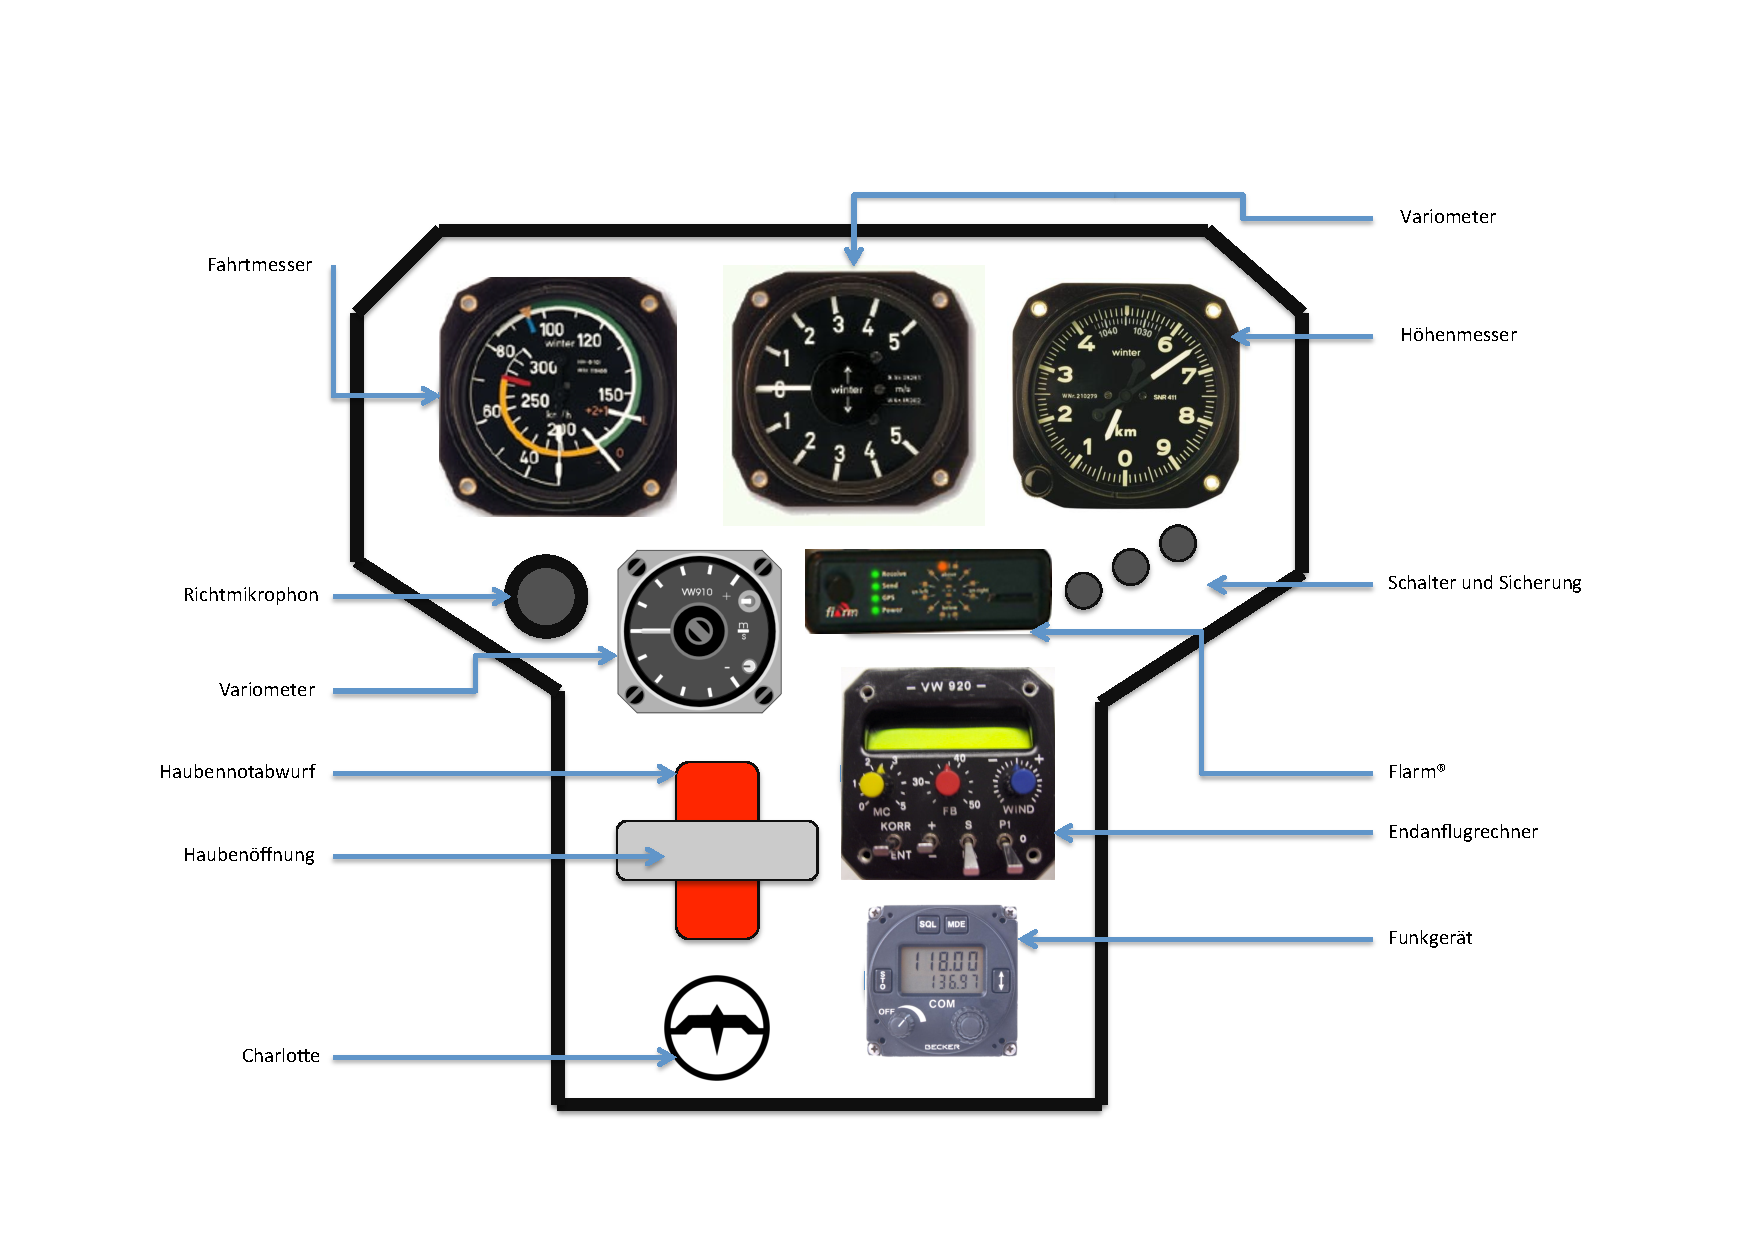
\includegraphics[angle=90,width=\textwidth]{bilder/instrumentenpilz.pdf}
\caption{Instrumentenpilz}
\end{figure}

\section{Bremsklappen}
Dreistöckige Bremsklappen auf der Oberseite des Innentragflügels. Der Antrieb mit Verknieung ist im Mittelrumpf angeordnet.

\section{Gepäckraum}
Das Gepäckfach befindet sich hinter dem rechten Piloten und hat eine maximale Zuladung von $\unit[10]{kg}$.

\section{Triebwerksanlage}
Eine detaillierte Beschreibung des FES Triebwerks ist im \textbf{FES WARTUNGSHANDBUCH} zu finden, wo auch die weiteren FES spezifischen Handbücher
aufgelistet sind.

\section{Akkupacks}
Eine detaillierte Beschreibung ist im \textbf{FES AKKUPACKSHANDBUCH} zu finden.

\section{Elektrische Anlage}
Eine detaillierte Beschreibung ist im \textbf{FES WARTUNGSHANDBUCH} zu finden.

\section{Sonstige Ausrüstung}
Eine detaillierte Beschreibung des FES BMS (Battery management system), FES Ladegerats und der BMS Steuerungssoftware ist im \textbf{FES AKKUPACKHANDBUCH} zu
finden.
